\documentclass[conference]{IEEEtran}
\usepackage[T1]{fontenc}
\usepackage{newtxtext,newtxmath}
\usepackage{cite}
\usepackage{amsmath}
\usepackage{balance}
\usepackage{graphicx}
\usepackage{textcomp}
\usepackage{xcolor}
\usepackage{booktabs}
\usepackage{multirow}
\usepackage{url}
\def\BibTeX{{\rm B\kern-.05em{\sc i\kern-.025em b}\kern-.08em
    T\kern-.1667em\lower.7ex\hbox{E}\kern-.125emX}}
\newcommand{\ms}{\,ms}
\newcommand{\us}{\,\textmu s}

\begin{document}

\title{Same Runtime, Same Speed? A Controlled Rust Versus C++ Comparison of ONNX Runtime Inference for Limit Order Book Prediction}

\author{\IEEEauthorblockN{Ujwal Akotkar}
\IEEEauthorblockA{\textit{Dept. of Computer Science and Engineering}\\
\textit{Indian Institute of Information Technology Dharwad}\\
Dharwad, India}
\and
\IEEEauthorblockN{Priyanshu Mittal}
\IEEEauthorblockA{\textit{Dept. of Data Science and Artificial Intelligence}\\
\textit{Indian Institute of Information Technology Dharwad}\\
Dharwad, India}
\and
\IEEEauthorblockN{Piyush Prashant}
\IEEEauthorblockA{\textit{Dept. of Data Science and Artificial Intelligence}\\
\textit{Indian Institute of Information Technology Dharwad}\\
Dharwad, India}
}

\maketitle

\begin{abstract}
Deep models for limit order book mid-price prediction are trained in Python but deployed through native inference runtimes, and Rust is increasingly proposed as a memory-safe replacement for C++ on that path. We present a controlled comparison of a Rust inference engine and an existing C++ engine for two published architectures, DeepLOB and a Transformer variant, on the FI-2010 benchmark. Both engines execute identical ONNX models on identical preprocessed inputs with the same ONNX Runtime release, and every measurement runs in a fresh process within a randomized, interleaved schedule of 499 processes. When both engines load the same vendor runtime library, their median latencies differ by at most 1.1 percent, their outputs are bit-identical, and the host languages add only microseconds per call. The differences that remain come from the deployment stack rather than the language: the runtime build bundled by the Rust binding is up to 55 percent slower with multi-threading, and the binding's default device policy silently offloads part of each model to Apple Core ML, which changes the outputs and doubles the latency. We release the benchmark harness, which detects both effects.
\end{abstract}

\begin{IEEEkeywords}
Rust, C++, ONNX Runtime, inference latency, limit order book, benchmarking methodology, reproducibility
\end{IEEEkeywords}

\section{Introduction}

Deep learning models such as DeepLOB~\cite{zhang2019deeplob} and Transformer-based variants~\cite{wallbridge2020translob} predict short-horizon mid-price movements from limit order book (LOB) snapshots, and FI-2010~\cite{ntakaris2018fi2010} is the standard benchmark for them. Such models are trained in Python, exported to ONNX, and served by a native runtime such as ONNX Runtime~\cite{onnxruntime}, where every additional microsecond counts against a trading latency budget. C++ is the conventional host language for this path; Rust offers memory safety without garbage collection~\cite{matsakis2014rust,jung2018rustbelt} and is increasingly proposed in its place.

Whether replacing a C++ engine with Rust costs latency, accuracy, or reproducibility is hard to judge from existing reports. Comparisons between language engines often differ in runtime version, thread configuration, inputs, and timer boundaries at the same time. Our own preliminary comparison had all four problems: a single-threaded C++ engine on ONNX Runtime 1.24 was timed on synthetic inputs, while a default-threaded Rust engine on version 1.31 was timed on dataset windows. Small benchmarking choices are known to produce misleading conclusions~\cite{mytkowicz2009wrong,georges2007rigorous,hoefler2015scientific}.

This paper isolates the host language. We compare RustLOB, a Rust engine built on the \texttt{ort} bindings~\cite{ort}, with the C++ engine of DeepLOB-HFT-Cpp~\cite{prashant2026deeplobhft}, and we make the following contributions.
\begin{itemize}
\item A controlled Rust versus C++ comparison on two LOB architectures with identical models, inputs, and runtime release, including a same-binary control that leaves the host language as the only difference.
\item Evidence that the remaining gaps are deployment-stack effects: the runtime build bundled by the Rust binding and the binding's implicit automatic device policy, confirmed with ONNX Runtime node-placement traces.
\item An open, process-isolated benchmark harness with numerical-equivalence and placement checks, together with a data audit that aligned both engines' windowing and labels with the training code.
\end{itemize}

\section{Background and Related Work}

\textit{LOB prediction.} Early work modelled LOB dynamics with support vector machines on hand-crafted features~\cite{kercheval2015svm}. Convolutional models~\cite{tsantekidis2017cnn} and DeepLOB, which combines convolutions with an LSTM~\cite{zhang2019deeplob}, became standard baselines on FI-2010, which contains ten days of order-book data for five Nasdaq Nordic stocks~\cite{ntakaris2018fi2010}. TransLOB replaced the recurrent encoder with self-attention~\cite{wallbridge2020translob,vaswani2017attention}. These works evaluate predictive accuracy; DeepLOB-HFT-Cpp~\cite{prashant2026deeplobhft} added a C++ ONNX Runtime deployment path and reported a 1.75-fold speed-up over Python.

\textit{Inference runtimes and host languages.} ONNX Runtime executes exported graphs through pluggable execution providers with configurable thread pools and graph optimizations~\cite{onnxruntime}. When different host languages call the same runtime, little of the per-call time is spent in the host: a recent industry study found Rust only 1.1 times faster than Python for a small model served through ONNX Runtime~\cite{qdrant2026oxidizing}. We test whether the same holds for Rust against C++, the stronger baseline.

\textit{Benchmarking methodology.} Process-level variation, warm-up, and measurement bias require repeated runs in fresh processes and statistics over runs rather than over correlated samples~\cite{georges2007rigorous,kalibera2013rigorous,hoefler2015scientific,mytkowicz2009wrong}. We follow these recommendations and compare per-process medians with the Mann--Whitney U test~\cite{mann1947test} and bootstrap confidence intervals~\cite{efron1993bootstrap}.

\section{Systems Under Test}

Table~\ref{tab:engines} lists the four configurations. All use ONNX Runtime 1.31.0 built from the same source commit, the CPU execution provider, batch size one, a float32 input of shape $1\times1\times100\times40$, zero-copy input tensors (a C++ \texttt{CreateTensor} over the window buffer and a borrowed Rust \texttt{TensorRef}), and an argmax over three logits.

\begin{table}[t]
\caption{Engine configurations (all ONNX Runtime 1.31.0, CPU)}
\label{tab:engines}
\centering
\footnotesize
\setlength{\tabcolsep}{3pt}
\begin{tabular}{@{}lll@{}}
\toprule
Configuration & Host API & Runtime library \\
\midrule
C++ & ORT C++ API & Microsoft, shared \\
Rust (bundled) & \texttt{ort} 2.0.0-rc.15 & \texttt{ort}-bundled, static \\
Rust (Microsoft) & \texttt{ort}, dynamic load & Microsoft, shared \\
Rust (default policy) & \texttt{ort}, implicit policy & \texttt{ort}-bundled, static \\
\bottomrule
\end{tabular}
\end{table}

\textit{C++ engine.} The C++ engine of~\cite{prashant2026deeplobhft} was built unmodified on macOS against Microsoft's ONNX Runtime 1.31.0 C++ SDK and reproduced its published TransformerLOB accuracy on its first 500 test windows exactly (165 of 500). For the benchmark, a thin adapter reuses its session setup and reads the shared input file.

\textit{Rust engine.} RustLOB is a 5,800-line Rust command-line engine that validates each model's input and output signature against the loaded ONNX graph, contains no \texttt{unsafe} code, and records the linked runtime build in every report. By default it links the ONNX Runtime build that the \texttt{ort} crate downloads; an optional feature loads any runtime library at start-up, which provides the same-binary control.

\textit{Models.} DeepLOB (three convolutional blocks and an LSTM, 69,507 parameters, ONNX opset 14) and TransformerLOB (the same convolutional front end and a two-layer, four-head Transformer encoder, 119,911 parameters, opset 18) were exported from PyTorch; both engines load byte-identical files.

\section{Methodology}

\textit{Data and audit.} We use the FI-2010 test split (31,937 rows), standardized with the training statistics shipped with the models. Window $i$ covers rows $i$ to $i+99$ and is labelled with row $i+100$, the convention of the training code. An audit of the data and of both engines against that code found three discrepancies in the Rust engine, all corrected before measurement. It labelled each window with its last row (a different label for 28\% of windows), used non-overlapping instead of stride-one windows, and named class 0 ``Down'' although FI-2010 label 1 denotes an upward move, which we confirmed against subsequent mid-price changes. After the corrections, both engines evaluate the same 31,837 windows of the raw test file and produce identical counts of correct predictions.

\textit{Protocol.} Latency is measured on 319 windows taken at stride 100; every engine reads the same exported tensor file. Each trial is a fresh operating-system process that performs 20 warm-up calls and 200 timed calls. Each configuration is repeated in 15 processes, and all configuration--repetition pairs are shuffled with a fixed seed and executed interleaved with a 1\,s pause, so slow drift affects all engines alike. The factors are engine, model, intra-op threads (one or the runtime default), and input policy (one window reused or all windows cycled; the two policies gave the same results, and we report cycled inputs). Each call records the full prediction path and, separately, the time spent in \texttt{Session::Run}. Cold start is the wall time from process creation to the first prediction and exit. Before timing, ONNX Runtime trace logs verify that CPU-only configurations place no node on another execution provider.

\textit{Statistics.} The unit of replication is a process. We summarize each configuration by the median of its 15 per-process medians and compare configurations with two-sided Mann--Whitney U tests on per-process medians~\cite{mann1947test}. The ratio of medians receives a 95\% bootstrap confidence interval from 10,000 resamples~\cite{efron1993bootstrap}. Tail percentiles are nearest-rank over all calls.

\textit{Platform.} An Apple M3 with four performance and four efficiency cores and 8\,GiB of memory, running macOS 26.5 on battery power with Low Power Mode disabled. Rust 1.97 and Apple Clang 17 were used in release mode.

\section{Results}

\subsection{Latency}

\begin{figure*}[t]
\centering
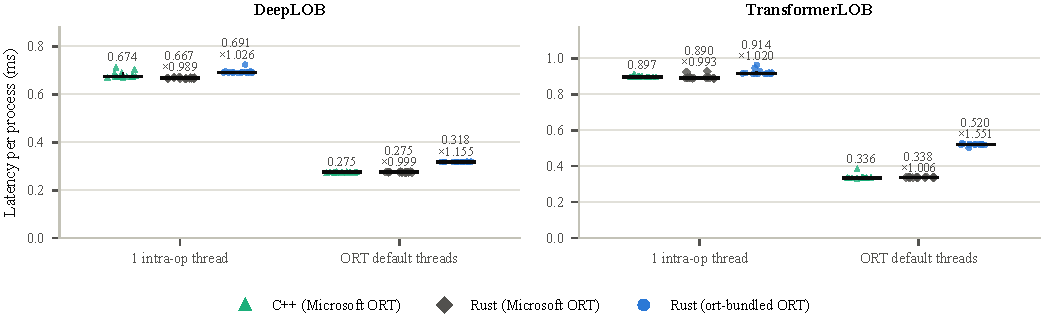
\includegraphics[width=\textwidth]{figures/fig_latency.pdf}
\caption{Per-process median latency (dots, 15 processes each), median of medians with 95\% bootstrap interval (bars), and ratio to C++ (labels). With the same Microsoft runtime library, Rust matches C++; with the runtime bundled by the \texttt{ort} crate it is slower, most visibly with the default thread pool.}
\label{fig:latency}
\end{figure*}

\begin{table*}[t]
\caption{Median of per-process median latency (ms, 15 processes each) and ratio to C++ with 95\% bootstrap CI and Mann--Whitney $p$}
\label{tab:latency}
\centering
\footnotesize
\setlength{\tabcolsep}{4pt}
\begin{tabular}{@{}llcccccccc@{}}
\toprule
 & & & \multicolumn{3}{c}{Rust (Microsoft runtime, same binary family)} & \multicolumn{3}{c}{Rust (\texttt{ort}-bundled runtime)} \\
\cmidrule(lr){4-6}\cmidrule(lr){7-9}
Model & Threads & C++ & Latency & Ratio [95\% CI] & $p$ & Latency & Ratio [95\% CI] & $p$ \\
\midrule
DeepLOB & 1 & 0.674 & 0.667 & 0.989 [0.971, 0.993] & $9\times10^{-6}$ & 0.691 & 1.026 [1.005, 1.028] & $6\times10^{-4}$ \\
DeepLOB & default & 0.275 & 0.275 & 0.999 [0.995, 1.002] & 0.25 & 0.318 & 1.155 [1.150, 1.157] & $3\times10^{-6}$ \\
TransformerLOB & 1 & 0.897 & 0.890 & 0.993 [0.992, 0.996] & $9\times10^{-4}$ & 0.914 & 1.020 [1.019, 1.026] & $5\times10^{-6}$ \\
TransformerLOB & default & 0.336 & 0.338 & 1.006 [1.003, 1.008] & 0.004 & 0.520 & 1.551 [1.543, 1.558] & $3\times10^{-6}$ \\
\bottomrule
\end{tabular}
\end{table*}

Fig.~\ref{fig:latency} and Table~\ref{tab:latency} summarize latency. With the same Microsoft runtime library on both sides, Rust and C++ differ by at most 1.1\%. Rust is slightly faster with one thread (DeepLOB $p=9\times10^{-6}$; TransformerLOB $p=9\times10^{-4}$); with the default thread pool there is no difference for DeepLOB ($p=0.25$) and C++ is 0.6\% faster for TransformerLOB ($p=0.004$). With the runtime build bundled by \texttt{ort}, Rust is 2.0--2.6\% slower than C++ with one thread and 15.5\% (DeepLOB) or 55.1\% (TransformerLOB) slower with the default thread pool ($p\le6\times10^{-4}$ for all four comparisons). Because the same Rust code linked against the Microsoft library closes the gap completely, the slowdown belongs to the bundled runtime build, not to Rust.

\subsection{Where the Time Goes}

The time spent per call outside \texttt{Session::Run} is 0.3--0.4\us\ for C++ and 1.8--2.2\us\ for Rust, which validates the input, creates a borrowed tensor view, checks the output shape and finiteness, and computes the argmax. In both engines this overhead is below 0.7\% of a call, so more than 99\% of the latency is spent inside the shared runtime. Disabling graph optimization slows the Rust engine by about 10\% (DeepLOB 0.763 versus 0.691\ms; TransformerLOB 1.011 versus 0.914\ms), an effect of the same order as the binary difference and far larger than the language effect.

\subsection{Tails, Throughput, and Cold Start}

\begin{figure}[t]
\centering
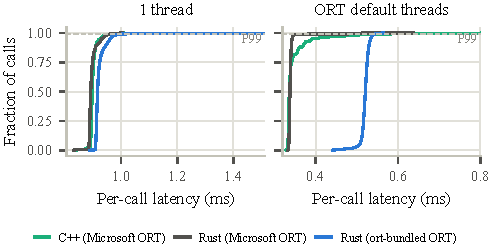
\includegraphics[width=\columnwidth]{figures/fig_ecdf.pdf}
\caption{Per-call latency distribution for TransformerLOB, pooled over 15 processes per configuration; the x-axis ends at the largest 99.9th percentile.}
\label{fig:ecdf}
\end{figure}

\begin{table}[t]
\caption{Tail latency (ms) and cold start of Rust (bundled) and C++}
\label{tab:tails}
\centering
\footnotesize
\setlength{\tabcolsep}{3.2pt}
\begin{tabular}{@{}llcccc@{}}
\toprule
 & & \multicolumn{2}{c}{C++} & \multicolumn{2}{c}{Rust} \\
\cmidrule(lr){3-4}\cmidrule(lr){5-6}
Model & Threads & P99 & P99.9 & P99 & P99.9 \\
\midrule
DeepLOB & 1 & 0.84 & 1.15 & 0.74 & 0.85 \\
DeepLOB & default & 0.37 & 0.51 & 0.35 & 0.42 \\
TransformerLOB & 1 & 0.96 & 1.00 & 1.00 & 1.47 \\
TransformerLOB & default & 0.53 & 0.78 & 0.54 & 0.56 \\
\midrule
\multicolumn{2}{@{}l}{Cold start, DeepLOB} & \multicolumn{2}{c}{42.4} & \multicolumn{2}{c}{36.9} \\
\multicolumn{2}{@{}l}{Cold start, TransformerLOB} & \multicolumn{2}{c}{55.4} & \multicolumn{2}{c}{50.7} \\
\bottomrule
\end{tabular}
\end{table}

Neither engine has systematically heavier tails (Fig.~\ref{fig:ecdf}, Table~\ref{tab:tails}): the 99th and 99.9th percentiles alternate between the two engines across configurations. Median throughput with one thread is 1,467 (C++) and 1,444 (Rust) windows per second for DeepLOB and 1,112 and 1,092 for TransformerLOB. Rust starts about 5\ms\ faster (Table~\ref{tab:tails}): its binary links the runtime statically, whereas the C++ engine loads a 45\,MB shared library at start-up.

\subsection{Numerical Equivalence}

On all 319 benchmark windows the three CPU configurations produce bit-identical logits with one intra-op thread. With the default thread pool, every configuration deviates from the single-thread result by the same amount, at most $5.4\times10^{-6}$, which reflects parallel reduction order and stays within a $10^{-5}$ tolerance; predicted classes agree for every window. On the complete test file (31,837 windows) both engines classify the same windows correctly: 18,908 for DeepLOB and 7,311 for TransformerLOB.

\subsection{A Deployment Pitfall: Implicit Device Policy}

\begin{table}[t]
\caption{Effect of the binding's implicit device policy (1 thread)}
\label{tab:coreml}
\centering
\footnotesize
\setlength{\tabcolsep}{3pt}
\begin{tabular}{@{}lcccc@{}}
\toprule
 & Core ML & Latency, ms & Max & Cold \\
Model & parts & (vs.\ C++) & $|\Delta|$ logit & start, ms \\
\midrule
DeepLOB & 2 of 7 & 0.797 ($\times$1.18) & $3.0\times10^{-3}$ & 117 \\
TransformerLOB & 14 of 51 & 1.770 ($\times$1.97) & $9.5\times10^{-4}$ & 442 \\
\bottomrule
\end{tabular}
\end{table}

Version 2.0.0-rc.15 of the \texttt{ort} crate sets ONNX Runtime's \textit{MaxEfficiency} automatic device policy on every session. On Apple silicon, the runtime then assigns fused partitions of both models to the Core ML execution provider, although only the CPU provider was registered and reports listed the provider as CPU (Table~\ref{tab:coreml}; parts are post-partitioning graph nodes). The offloaded configuration changes logits by up to $3\times10^{-3}$, 300 times the tolerance, is up to 1.97 times slower than C++, and starts up to eight times slower than the CPU configuration because of Core ML model compilation. The C++ API applies no such policy. Selecting the \textit{PreferCPU} policy restores bit-identical outputs and C++-level latency; RustLOB now does so by default and checks the placement in its tests.

\section{Discussion}

\textit{Language is not the bottleneck.} For models of this size, each prediction takes 0.3--0.9\ms, of which more than 99\% is spent in the shared runtime; the host language contributes microseconds. With identical runtime binaries, the Rust and C++ engines are equivalent for practical purposes, and Rust's memory safety and statically linked single binary come at no measurable inference cost.

\textit{The deployment stack is.} Two binding-level defaults dominate the differences we observed: which runtime binary is linked (2--55\% here, largest with multi-threading) and which devices the runtime may use (a silent change of hardware and numerical precision). Neither is visible in application code. Both were found only through a same-binary control and node-placement traces, and either would have been misattributed to the language in a conventional comparison.

\textit{Recommendations.} Record the exact runtime binary rather than only its version; pin the execution provider and verify node placement; compare engines on the same runtime binary; run each trial in a fresh process within an interleaved schedule; and report statistics over processes rather than over pooled calls.

\textit{Threats to validity.} All measurements come from one machine (an Apple M3 with macOS), on the CPU, at batch size one, on battery power; an x86-64 Linux platform should be added before generalizing. The two Microsoft libraries are separately packaged builds of the same release. Both models are small (under 120,000 parameters), so the language share of latency is likely to shrink further for larger models. Earlier runs on the same machine showed an engine-independent bimodal process state (per-process medians about 1.7 times apart, equally frequent for all engines); it did not occur in the final run, and all comparisons come from one interleaved schedule. Predictive quality is outside the scope of this study because both engines execute the same files: the models reach 59.4\% (DeepLOB) and 23.0\% (TransformerLOB) accuracy on the full test file, and the normalization statistics shipped with them differ from those used in training.

\section{Conclusion}

Under controlled conditions, with identical models, inputs, runtime release, and runtime binary, a Rust ONNX Runtime engine matches a C++ engine within 1.1\% for DeepLOB and TransformerLOB inference, produces bit-identical outputs, and adds only microseconds of per-call overhead. The performance and correctness risks lie in the deployment stack: the runtime binary that a binding ships and the device policy it applies by default. The benchmark harness, both engines, and all results are publicly available.\footnote{\raggedright\url{https://github.com/kairx007/rust-onxx-engine}, branch \texttt{feat/phase2-benchmarking}.}

\balance
\begin{thebibliography}{00}
\bibitem{zhang2019deeplob} Z. Zhang, S. Zohren, and S. Roberts, ``DeepLOB: Deep convolutional neural networks for limit order books,'' \textit{IEEE Trans. Signal Process.}, vol. 67, no. 11, pp. 3001--3012, 2019.
\bibitem{ntakaris2018fi2010} A. Ntakaris, M. Magris, J. Kanniainen, M. Gabbouj, and A. Iosifidis, ``Benchmark dataset for mid-price forecasting of limit order book data with machine learning methods,'' \textit{J. Forecasting}, vol. 37, no. 8, pp. 852--866, 2018.
\bibitem{wallbridge2020translob} J. Wallbridge, ``Transformers for limit order books,'' arXiv:2003.00130, 2020.
\bibitem{tsantekidis2017cnn} A. Tsantekidis, N. Passalis, A. Tefas, J. Kanniainen, M. Gabbouj, and A. Iosifidis, ``Forecasting stock prices from the limit order book using convolutional neural networks,'' in \textit{Proc. IEEE Conf. Business Informatics (CBI)}, 2017.
\bibitem{kercheval2015svm} A. N. Kercheval and Y. Zhang, ``Modelling high-frequency limit order book dynamics with support vector machines,'' \textit{Quantitative Finance}, vol. 15, no. 8, pp. 1315--1329, 2015.
\bibitem{vaswani2017attention} A. Vaswani \textit{et al.}, ``Attention is all you need,'' in \textit{Proc. NeurIPS}, 2017, pp. 5998--6008.
\bibitem{prashant2026deeplobhft} P. Prashant, P. Mittal, H. M. S., Monika, and V. Poddar, ``DeepLOB-HFT-Cpp: A production-grade deep learning pipeline for limit order book mid-price prediction with high-performance C++ inference,'' Indian Inst. Inf. Technol. Dharwad, unpublished manuscript, 2026.
\bibitem{onnxruntime} ONNX Runtime developers, ``ONNX Runtime,'' 2021. [Online]. Available: \url{https://onnxruntime.ai}
\bibitem{ort} pyke.io, ``ort: Rust bindings for ONNX Runtime,'' [Online]. Available: \url{https://github.com/pykeio/ort}
\bibitem{matsakis2014rust} N. D. Matsakis and F. S. Klock II, ``The Rust language,'' \textit{ACM SIGAda Ada Letters}, vol. 34, no. 3, pp. 103--104, 2014.
\bibitem{jung2018rustbelt} R. Jung, J.-H. Jourdan, R. Krebbers, and D. Dreyer, ``RustBelt: Securing the foundations of the Rust programming language,'' \textit{Proc. ACM Program. Lang.}, vol. 2, no. POPL, art. 66, 2018.
\bibitem{qdrant2026oxidizing} Qdrant, ``Oxidizing cross-encoders,'' 2026. [Online]. Available: \url{https://qdrant.tech/blog/oxidizing-cross-encoders/}
\bibitem{georges2007rigorous} A. Georges, D. Buytaert, and L. Eeckhout, ``Statistically rigorous Java performance evaluation,'' in \textit{Proc. OOPSLA}, 2007, pp. 57--76.
\bibitem{mytkowicz2009wrong} T. Mytkowicz, A. Diwan, M. Hauswirth, and P. F. Sweeney, ``Producing wrong data without doing anything obviously wrong!'' in \textit{Proc. ASPLOS}, 2009, pp. 265--276.
\bibitem{kalibera2013rigorous} T. Kalibera and R. Jones, ``Rigorous benchmarking in reasonable time,'' in \textit{Proc. ISMM}, 2013, pp. 63--74.
\bibitem{hoefler2015scientific} T. Hoefler and R. Belli, ``Scientific benchmarking of parallel computing systems: Twelve ways to tell the masses when reporting performance results,'' in \textit{Proc. SC}, 2015, art. 73.
\bibitem{mann1947test} H. B. Mann and D. R. Whitney, ``On a test of whether one of two random variables is stochastically larger than the other,'' \textit{Ann. Math. Statist.}, vol. 18, no. 1, pp. 50--60, 1947.
\bibitem{efron1993bootstrap} B. Efron and R. J. Tibshirani, \textit{An Introduction to the Bootstrap}. New York, NY, USA: Chapman \& Hall, 1993.
\end{thebibliography}

\end{document}
